\begin{LQ}{Cas d'utilisation}

\LQDescription{
    Les cas d'utilisation sont la description d'une suite d'interactions entre
    des acteurs (humains ou non) et un système. Ils sont représentés
    graphiquement par des diagrammes de cas d'utilisation. Les cas
    d'utilisation doivent repondre à un besoin clairement expliciter dans le
    cahier des charges.
}

\LQSchema{
    On definit d'abord le périmètre du système par un rectangle en mettant le
    nom de ce système en haut de ce rectangle.  Les acteurs du CdU sont
    représenter par des "bonhommes" quelque soit leur nature. On met par
    convention les acteurs physiques à gauche et les acteurs de type système à
    droite. Les interactions entre les différents acteurs sont les Cdu que l'on
    modélise par une action  que l'on met dans une bulle. Les différents
    acteurs sont liés par ces actions.
}

\begin{figure}[H]
   \centering
   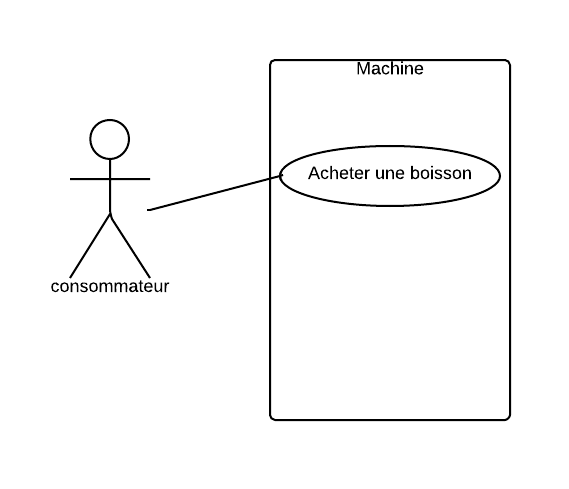
\includegraphics[width=\textwidth]{images/CdU.png}
   \caption{Schéma des cas d'utilisation}
\end{figure}

\LQModel{
    Chaque cas d'utilisation doit être structuré de façon à constituer une
    spécification complète et intuitive des fonctionnalités. \\

    Il faut veiller à ce que les extensions/dysfonctionnement découlent
    toujours d'une étape du scénario établi. \\

    Il faut essayer de trouver un bon niveau de détails pour le CdU. On doit
    être ni trop précis, ni trop vague. La difficulté est de pouvoir être
    concis sans rentrer dans trop de details. Il est conseillé de commencer de
    manière abstraite et d'affinité ces modèles au fur et à mesure. Si on
    arrive à plus de 15 CdU, on estime que la précisions est trop importante.
    Cela signifie que certaine tache peuvent sûrement être regroupé entre
    elle. \\

    Le CdU doit être compréhensible par le client donc le choix des nom des
    acteurs et de l'ensemble des éléments du schéma doit être clair et simple.
    Le langage ne doit pas être technique.\\

    Il ne faut pas décrire les interaction entre les acteurs. Un CdU décrit les
    interactions entre les acteurs et le système. \\

    Attention à bien choisir les acteurs. Un acteur ne doit pas être interne au
    système. Il doit profiter de l'utilisation du système, et interagir
    directement avec lui. Il est plus un rôle,
    un profil, qu'une entité physique concrète.
}

\LQBetweenModels{
    Si un cas d'utilisation possède une pré-condition, il faut s'assurer qu'il
    existe un autre cas d'utilisation  qui possède une post-condition
    identique. \\

    Les cas d'utilisation doivent rester autant que possible indépendants les
    uns des autres. Il faut éviter de se perdre dans les détails quant aux
    interférences, à la concurrence et aux conflits entre cas d'utilisation.
}

\end{LQ}
